\documentclass[a4paper]{article}

\usepackage{fullpage} % Package to use full page
\usepackage{parskip} % Package to tweak paragraph skipping
\usepackage{tikz} % Package for drawing

\usepackage{hyperref}
\usepackage{amsmath}
\usepackage{amssymb}
\usepackage{amsthm}
\usepackage{enumitem}

\usepackage{subcaption}

\title{COMP 339 Assignment 4}
\author{Ling Tan}
\date{2018/11/13}

\begin{document}

\maketitle

\section{}
\begin{enumerate}[label=\alph*)]
      \item Show that the Petersen graph has no Hamilton cycle but that is has a Hamilton path.\\
          \textcolor{blue}{Answer:}\\
          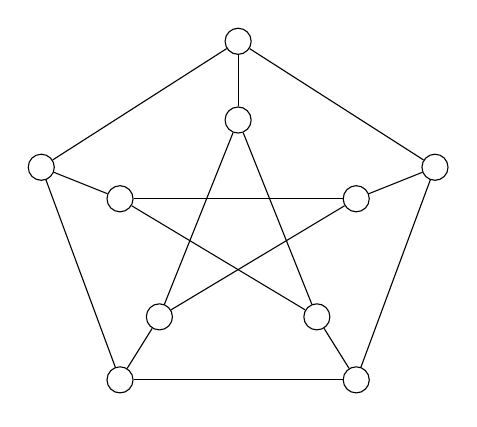
\begin{tikzpicture}[auto]
                \begin{scope}[every node/.style={circle,draw=black}]
                    \node (A) at (0,0) {};
                    \node (B) at (1.5,-1) {};
                    \node (C) at (1,-2.5) {};
                    \node (D) at (-1,-2.5) {};
                    \node (E) at (-1.5,-1) {};
                    \node (A1) at (0,1) {};
                    \node (B1) at (2.5,-0.6) {};
                    \node (C1) at (1.5,-3.3) {};
                    \node (D1) at (-1.5,-3.3) {};
                    \node (E1) at (-2.5,-0.6) {};
                \end{scope}
                \begin{scope}[every edge/.style={draw=black}]
                    \draw (A) edge node{} (C);
                    \draw (A) edge node{} (D);
                    \draw (B) edge node{} (D);
                    \draw (B) edge node{} (E);
                    \draw (E) edge node{} (C);
                    \draw (A1) edge node{} (B1);
                    \draw (B1) edge node{} (C1);
                    \draw (C1) edge node{} (D1);
                    \draw (D1) edge node{} (E1);
                    \draw (E1) edge node{} (A1);
                    \draw (A) edge node{} (A1);
                    \draw (B) edge node{} (B1);
                    \draw (C) edge node{} (C1);
                    \draw (D) edge node{} (D1);
                    \draw (E) edge node{} (E1);
                \end{scope}
            \end{tikzpicture}\\
            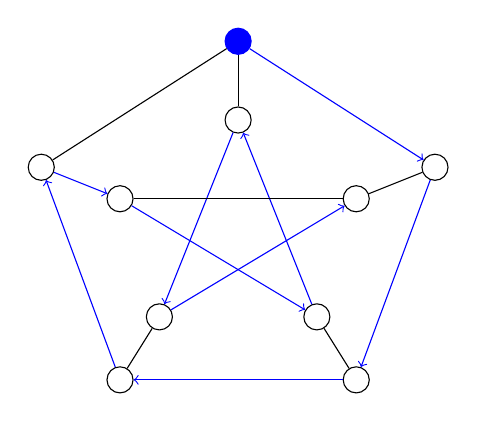
\begin{tikzpicture}[auto]
                \begin{scope}[every node/.style={circle,draw=black}]
                    \node (A) at (0,0) {};
                    \node (B) at (1.5,-1) {};
                    \node (C) at (1,-2.5) {};
                    \node (D) at (-1,-2.5) {};
                    \node (E) at (-1.5,-1) {};
                    \node (A1) [fill, blue] at (0,1) {};
                    \node (B1) at (2.5,-0.6) {};
                    \node (C1) at (1.5,-3.3) {};
                    \node (D1) at (-1.5,-3.3) {};
                    \node (E1) at (-2.5,-0.6) {};
                \end{scope}
                \begin{scope}[every edge/.style={draw=black}]
                    \draw (A) edge [<-, blue] node{} (C);
                    \draw (A) edge [->, blue] node{} (D);
                    \draw (B) edge [<-, blue] node{} (D);
                    \draw (B) edge node{} (E);
                    \draw (E) edge [->, blue] node{} (C);
                    \draw (A1) edge [->, blue] node{} (B1);
                    \draw (B1) edge [->, blue] node{} (C1);
                    \draw (C1) edge [->, blue] node{} (D1);
                    \draw (D1) edge [->, blue] node{} (E1);
                    \draw (E1) edge node{} (A1);
                    \draw (A) edge node{} (A1);
                    \draw (B) edge node{} (B1);
                    \draw (C) edge node{} (C1);
                    \draw (D) edge node{} (D1);
                    \draw (E) edge [<-, blue] node{} (E1);
                \end{scope}
            \end{tikzpicture}
      \item Show that if any vertex (and the edges incident to it) is removed from the Petersen graph, then the resulting subgraph has a Hamilton cycle.\\
          \textcolor{blue}{Answer:}
          Because the Petersen graph is symmetric, we only have two cases:\\
          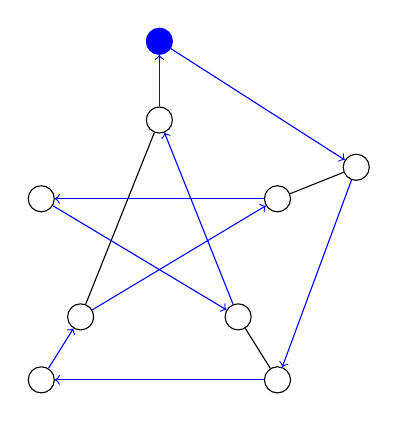
\begin{tikzpicture}[auto]
                \begin{scope}[every node/.style={circle,draw=black}]
                    \node (A) at (0,0) {};
                    \node (B) at (1.5,-1) {};
                    \node (C) at (1,-2.5) {};
                    \node (D) at (-1,-2.5) {};
                    \node (E) at (-1.5,-1) {};
                    \node (A1) [fill, blue] at (0,1) {};
                    \node (B1) at (2.5,-0.6) {};
                    \node (C1) at (1.5,-3.3) {};
                    \node (D1) at (-1.5,-3.3) {};
                \end{scope}
                \begin{scope}[every edge/.style={draw=black}]
                    \draw (A) edge [<-, blue] node{} (C);
                    \draw (A) edge node{} (D);
                    \draw (B) edge [<-, blue] node{} (D);
                    \draw (B) edge [->, blue] node{} (E);
                    \draw (E) edge [->, blue] node{} (C);
                    \draw (A1) edge [->, blue] node{} (B1);
                    \draw (B1) edge [->, blue] node{} (C1);
                    \draw (C1) edge [->, blue] node{} (D1);
                    \draw (A) edge [->, blue] node{} (A1);
                    \draw (B) edge node{} (B1);
                    \draw (C) edge node{} (C1);
                    \draw (D) edge [<-, blue] node{} (D1);
                \end{scope}
            \end{tikzpicture}
            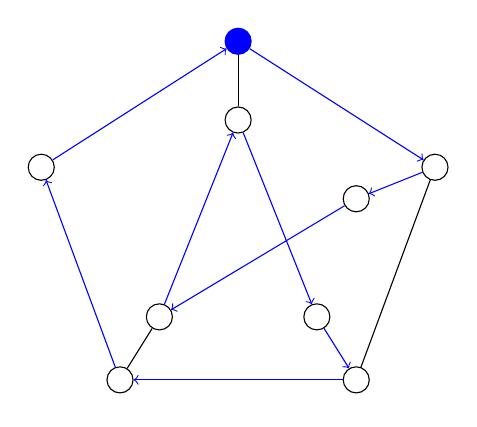
\begin{tikzpicture}[auto]
                \begin{scope}[every node/.style={circle,draw=black}]
                    \node (A) at (0,0) {};
                    \node (B) at (1.5,-1) {};
                    \node (C) at (1,-2.5) {};
                    \node (D) at (-1,-2.5) {};
                    \node (A1) [fill, blue] at (0,1) {};
                    \node (B1) at (2.5,-0.6) {};
                    \node (C1) at (1.5,-3.3) {};
                    \node (D1) at (-1.5,-3.3) {};
                    \node (E1) at (-2.5,-0.6) {};
                \end{scope}
                \begin{scope}[every edge/.style={draw=black}]
                    \draw (A) edge [->, blue] node{} (C);
                    \draw (A) edge [<-, blue] node{} (D);
                    \draw (B) edge [->, blue] node{} (D);
                    \draw (A1) edge [->, blue] node{} (B1);
                    \draw (B1) edge node{} (C1);
                    \draw (C1) edge [->, blue] node{} (D1);
                    \draw (D1) edge [->, blue] node{} (E1);
                    \draw (E1) edge [->, blue] node{} (A1);
                    \draw (A) edge node{} (A1);
                    \draw (B) edge [<-, blue] node{} (B1);
                    \draw (C) edge [->, blue] node{} (C1);
                    \draw (D) edge node{} (D1);
                \end{scope}
            \end{tikzpicture}
\end{enumerate}

\section{}
Find a counterexample to the converse of Theorem 11.8.

\section{}
Let $G=(V,E)$ be a loop-free undirected $n$-regular graph with $|V|\geq 2n+2$. Prove that $\Bar{G}$ has a Hamilton cycle.
\textcolor{blue}{Answer:}

\section{}
Let $n\in\mathbb{Z}^+$ with $n\geq 4$, and let the vertex set $V'$ for the complete graph $K_{n-1}$ be $\{v_1,v_2,\ldots, v_{n-1}\}$. Now construct the loop-free undirected graph $G_n=(V,E)$ from $K_{n-1}$ as follows: $V=V'\cup\{v\}$, and $E$ consists of all the edges in $K_{n-1}$ except for the edge $\{v_1,v_2\}$\, which is replaced by the pair of edges $\{v_1,v\}$ and $\{v,v_2\}$.
    \begin{enumerate}[label=\alph*)]
        \item Determine $deg(x)+deg(y)$ for all nonadjacent vertices $x$ and $y$ in $V$.
        \item Does $G_n$ have a Hamilton cycle?
        \item How large is the edge set $E$?
        \item Do the results in parts (b) and (c) contradict Corollary 11.6?
    \end{enumerate}
    \textcolor{blue}{Answer:}

\section{}
If $G$ is a loop-free undirected graph with at least one edge, prove that $G$ is bipartite if and only if $\chi(G)=2$.
    \textcolor{blue}{Answer:}
    
\section{}
Consider the complete graph $K_n$ for $n\geq 3$. Color $r$ of the vertices in $K_n$ red and the remaining $n-r(=g)$ vertices green. For any two vertices $v,w$ in $K_n$ color the edge $\{v,w\}$ (1) red if $v,w$ are both red;(2) green if $v,w$ are both green; or (3) blue if $v,w$ have different colors. Assume that $r\geq g$.
    \begin{enumerate}[label=\alph*)]
        \item Show that for $r=6$ and $g=3$ (and $n=9$) the total number of red and green edges in $K_9$ equals the number of blue edges in $K_9$.
        \item Show that the total number of red and green edges in $K_n$ equals the number of blue edges in $K_n$ if and only if $n=r+g$, where $g,r$ are consecutive triangular numbers. [The triangular numbers are defined recursively by $t_1=1, t_{n+1}=t_n+(n+1), n\geq 1$; so $t_n=n(n+1)/2$. hence $t_1=1,t_2=3,t+3=6,\ldots$.] 
    \end{enumerate}

\section{}
Let $G$ be a loop-free undirected graph, where $\Delta=\max_{v\in V}\{deg(v)\}$.
    \begin{enumerate}
        \item Prove that $\chi(G)\leq\Delta+1$.
        \item Find two types of graphs $G$, where $\chi(G)=\Delta+1$.
    \end{enumerate}

\section{}
\begin{enumerate}[label=\alph*)]
    \item If a tree has four vertices of degree $2$, one vertex of degree $3$, two degree of $4$, and one of degree $5$, how many pendant vertices does it have?
    \item If a tree $T=(V,E)$ has $v_2$ vertices of degree of $2$, $v_3$ vertices of degree $3,\ldots,$ and $v_m$ vertices of degree $m$, what are $|V|$ and $|E|$?
\end{enumerate}
\section{}
The connected undirected graph $G=(V,E)$ has $30$ edges. What is the maximum value that $|V|$ can have?\\
 \textcolor{blue}{Answer:} 
 
\section{}
Let $G=(V,E)$ be a loop-free connected undirected graph where $V=\{v_1,v_2,\ldots, v_n\}, n\geq2,deg(v_1)=1$, and $deg(v_i)\geq 2$ for $2\leq i\leq n$. Prove that $G$ must have a cycle.\\
\textcolor{blue}{Answer:}

\section{}
Does there exist a graph on $5$ vertices with the vertex degrees $4,4,3,2,2$?\\
\textcolor{blue}{Answer:} 

\section{}
Prove that in any tree there are two vertices of the same degree \\
\textcolor{blue}{Answer:} 
\begin{proof} By contradiction.\\
\end{proof}

\section{}
Prove that any undirected, loop-free graph on $n$ vertices with at least $(n-1)(n-2)/2 + 1$ edges is connected. Also, give
an example of a disconnected $n$-vertex graph with one fewer edge.\\
\textcolor{blue}{Answer:} 


\section{}
Which complete bipartite graphs $K_{m,n}$ have Hamilton cycles? Which have Hamilton paths?\\

\textcolor{blue}{Answer:} 
\end{document}

